\documentclass[11pt]{article}
\usepackage{amsmath, amssymb, amsthm}
\usepackage{geometry}
\usepackage{graphicx}
\geometry{margin=1in}
\setlength\parindent{0pt}
\title{Foundations of Machine Learning -- Neural Networks}
\author{}
\date{}

\begin{document}
\maketitle


\section*{Reinforcement Networks}

Reinforcement learning: An agent interacts with an environment via actions that change the state of the environment 
to maximize some notion of a cumulative reward.

\begin{figure}[h]
	\centering
	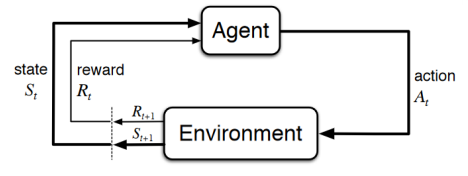
\includegraphics[width=0.5\textwidth]{../imgs/rein_learn.png}  
\end{figure}

Reinforcement learning requires many trials and errors and having a simulated environment is crucial.

\medskip

The main challenge in RL is improving the learning speed, and overcoming the gap between simulation and the real world. 

\subsection*{Reinforcement Learning Interaction Loop}

Reinforcement learning is defined by the interaction between an \emph{agent} and an \emph{environment}.  
At each discrete time step $t$, the following sequence occurs:

\begin{figure}[h]
	\centering
	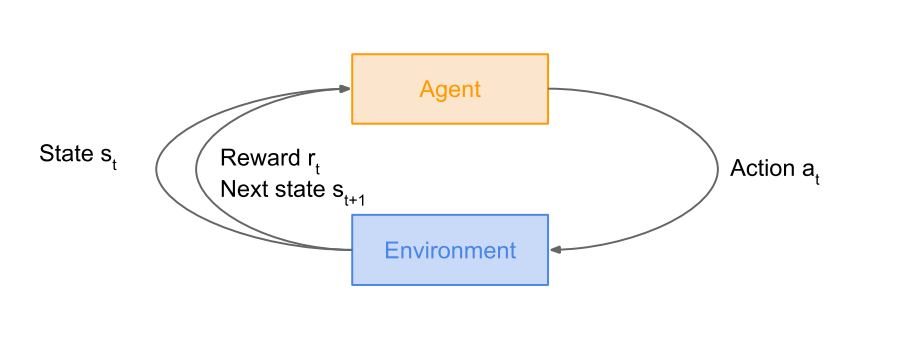
\includegraphics[width=0.5\textwidth]{../imgs/rein_learn_proc.png}  
\end{figure}

\begin{enumerate}
    \item \textbf{State Observation}  
    The environment presents the agent with a state
    \[
        s_t \in \mathcal{S}.
    \]

    \item \textbf{Action Selection}  
    Based on the current state, the agent selects an action
    \[
        a_t \in \mathcal{A},
    \]
    according to its policy $\pi(a_t \mid s_t)$.

    \item \textbf{Environment Transition}  
    After receiving the action, the environment generates:
    \begin{itemize}
        \item a scalar reward
        \[
            r_t = r(s_t, a_t),
        \]
        which evaluates the immediate utility of the action;
        \item the next state
        \[
            s_{t+1} \sim P(\cdot \mid s_t, a_t),
        \]
        where $P$ is the transition distribution.
    \end{itemize}

    \item \textbf{Learning Signal}  
    The tuple
    \[
        (s_t, a_t, r_t, s_{t+1})
    \]
    forms the fundamental data used by RL algorithms to update the policy or value function.
\end{enumerate}

The cycle then repeats for $t = 0, 1, 2, \ldots$ until a terminal state is reached or the episode ends.
This process defines a Markov Decision Process (MDP), which provides the formal foundation for  
value-based methods (e.g., Q-learning, DQN) and policy-based methods.


\subsection*{Markov Decision Process}

This gives us a way to mathematically formalize our RL problem from above and is defined by several properties.

\[
(\mathcal{S}, \mathcal{A}, \mathcal{R}, \mathcal{P}, \gamma)
\]

\begin{itemize}
    \item $\mathcal{S}$ : set of possible states
    \item $\mathcal{A}$ : set of possible actions
    \item $\mathcal{R}$ : distribution of reward given a \((\text{state}, \text{action})\) pair
    \item $\mathcal{P}$ : transition probability, i.e.\ distribution over next state given a \((\text{state}, \text{action})\) pair
    \item $\gamma$ : discount factor
\end{itemize}

\paragraph*{Markov Property}

This means that the future and the past are conditionally independent, given the present. This means 
the future depends only on the present state and action, not on the past.

\medskip

To express this mathematically, consider an agent that has visited states 
\(s_0, s_1, \ldots, s_t\) after taking actions 
\(a_0, a_1, \ldots, a_{t-1}\) in some MDP, and has just taken action \(a_t\).
The probability that the agent then arrives at state \(s_{t+1}\),
given the full history of previous states and actions, can be written as:

\[
P(S_{t+1} = s_{t+1} \mid 
S_t = s_t, A_t = a_t, 
S_{t-1} = s_{t-1}, A_{t-1} = a_{t-1}, 
\ldots, 
S_0 = s_0).
\]

Here, \(S_t\) denotes the random variable representing the agent's state at time \(t\),
and \(A_t\) denotes the random variable representing the action taken at time \(t\).

The Markov property states that this probability simplifies to:

\[
P(S_{t+1} = s_{t+1} \mid 
S_t = s_t, A_t = a_t, 
S_{t-1} = s_{t-1}, A_{t-1} = a_{t-1}, 
\ldots, 
S_0 = s_0)
=
P(S_{t+1} = s_{t+1} \mid S_t = s_t, A_t = a_t).
\]

\pagebreak

\paragraph*{Markov Decision Process}

A policy $\pi$ is a function from $\mathcal{S}$ to $\mathcal{A}$ that specifies what action to take in each state.



\begin{itemize}
    \item At time step $t = 0$, the environment samples an initial state 
    \[
        s_0 \sim p(s_0).
    \]

    \item Then, for $t = 0$ until the process terminates:
    \begin{itemize}
        \item Agent selects action $a_t$
        \item Environment samples reward 
        \[
            r_t \sim R(\,\cdot \mid s_t, a_t)
        \]
        \item Environment samples next state 
        \[
            s_{t+1} \sim P(\,\cdot \mid s_t, a_t)
        \]
        \item Agent receives reward $r_t$ and next state $s_{t+1}$
    \end{itemize}
  

\end{itemize}

\medskip

Our objective is to find a policy $\pi^*$ that maximizeds cumulative discounted reward:
\[
\sum_{t=0}^{\infty} \gamma^t r_t.
\]


\begin{figure}[!ht]
    \centering
    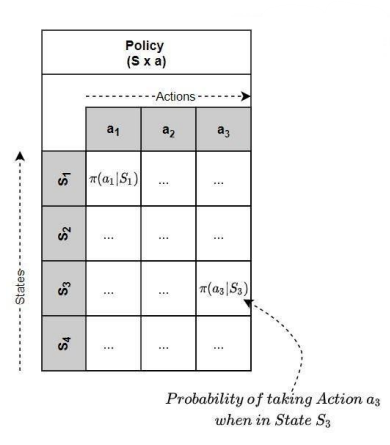
\includegraphics[width=0.55\textwidth]{../imgs/policy_grid.png}
\end{figure}

\pagebreak

\paragraph*{MDP Example (Grid World)}

\[
\mathcal{A} = \{\text{right}, \text{left}, \{\text{up}, \{\text{down}
\]

% \begin{figure}[!ht]
%     \centering
%     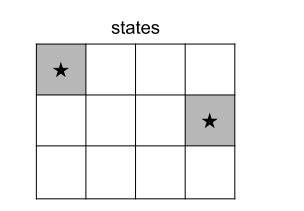
\includegraphics[width=0.25\textwidth]{../imgs/states_ex_blank.png}
% \end{figure}

\begin{figure}[!ht]
    \centering
    \hfill
    \begin{minipage}[b]{0.32\textwidth}
        \centering
        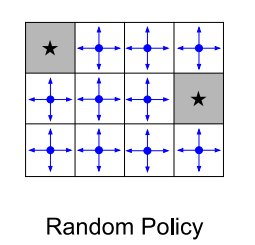
\includegraphics[width=\textwidth]{../imgs/states_ex_random.png}
    \end{minipage}
    \hfill
    \begin{minipage}[b]{0.32\textwidth}
        \centering
        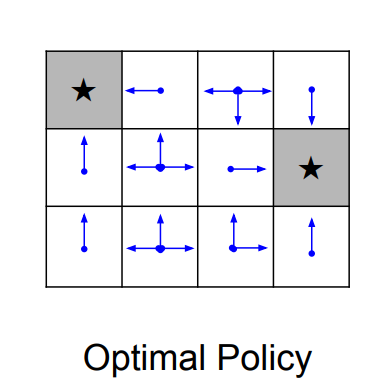
\includegraphics[width=\textwidth]{../imgs/states_ex_optimal.png}
    \end{minipage}
\end{figure}

Revisiting our optimal policy, we want to maximize the total sum of rewards, formally this is written as: 
\[
\pi^{*} = \arg\max_{\pi} \mathbb{E}\!\left[ \sum_{t \ge 0} \gamma^{t} r_{t} \,\middle|\, \pi \right]
\quad \text{with} \quad
s_{0} \sim p(s_{0}),\;
a_{t} \sim \pi(\cdot \mid s_{t}),\;
s_{t+1} \sim p(\cdot \mid s_{t}, a_{t}).
\]

\subsection*{Definitions: Value Function and Q-Value Function}



The \textbf{value function} at state \(s\) is the expected cumulative reward from following the policy starting from state \(s\):
\[
V^{\pi}(s) = 
\mathbb{E} \!\left[ \sum_{t \ge 0} \gamma^{t} r_t \,\middle|\, s_0 = s,\, \pi \right].
\]

This is answering, How good is it to be in the state s?

\medskip

The \textbf{Q-value function} at state \(s\) and action \(a\) is the expected cumulative reward from taking action \(a\) in state \(s\) and then following the policy:
\[
Q^{\pi}(s, a) = 
\mathbb{E} \!\left[ \sum_{t \ge 0} \gamma^{t} r_t \,\middle|\, s_0 = s,\; a_0 = a,\; \pi \right].
\]
This is answering, how good is it to be in the state s and take an action a in this state?

\pagebreak

\subsection*{Bellman Equation}

The optimal Q-value function \(Q^{*}\) is the maximum expected cumulative reward
achievable from a given \((\text{state}, \text{action})\) pair:


\[
Q^{*}(s, a)
    = \max_{\pi} 
        \mathbb{E} \!\left[
            \sum_{t \ge 0} \gamma^{t} r_t \,\middle|\,
            s_0 = s,\; a_0 = a,\; \pi
        \right].
\]

\(Q^{*}\) satisfies the following \textbf{Bellman equation}:

\[
Q^{*}(s, a)
    = \mathbb{E}_{s' \sim \mathcal{E}} 
        \left[
            r + \gamma \max_{a'} Q^{*}(s', a')
            \,\middle|\, s, a
        \right].
\]

\begin{itemize}
    \item $r(s,a)$ is the immediate reward for taking action $a$ in state $s$.
    \item $\gamma$ is the discount factor, which prioritizes near-term rewards over distant future rewards.
    \item $\max_{a'} Q^{*}(s',a')$ represents the maximum expected cumulative reward achievable from the next state $s'$, assuming the agent follows the optimal policy from there.
\end{itemize}

If we have $Q^{*}$, the Q-value function for the optimal policy $\pi^{*}$, we can obtain the optimal policy by
\[
\pi^{*}(s) = \arg\max_{a} Q^{*}(s,a).
\]
aka for each state pick the action with the highest Q-value


\pagebreak

\paragraph*{Car Example}

\[
\mathcal{S} = \{\text{cool}, \text{warm}, \text{overheated}\}, \qquad
\mathcal{A} = \{\text{slow}, \text{fast}\}
\]

Transition Function: $T(s, a, s')$

\begin{align*}
T(\text{cool}, \text{slow}, \text{cool}) &= 1 \\
T(\text{warm}, \text{slow}, \text{cool}) &= 0.5 \\
T(\text{warm}, \text{slow}, \text{warm}) &= 0.5 \\
T(\text{cool}, \text{fast}, \text{cool}) &= 0.5 \\
T(\text{cool}, \text{fast}, \text{warm}) &= 0.5 \\
T(\text{warm}, \text{fast}, \text{overheated}) &= 1
\end{align*}

Reward Function: $R(s, a, s')$

\begin{align*}
R(\text{cool}, \text{slow}, \text{cool}) &= 1 \\
R(\text{warm}, \text{slow}, \text{cool}) &= 1 \\
R(\text{warm}, \text{slow}, \text{warm}) &= 1 \\
R(\text{cool}, \text{fast}, \text{cool}) &= 2 \\
R(\text{cool}, \text{fast}, \text{warm}) &= 2 \\
R(\text{warm}, \text{fast}, \text{overheated}) &= -10
\end{align*}

\begin{figure}[h]
    \centering
    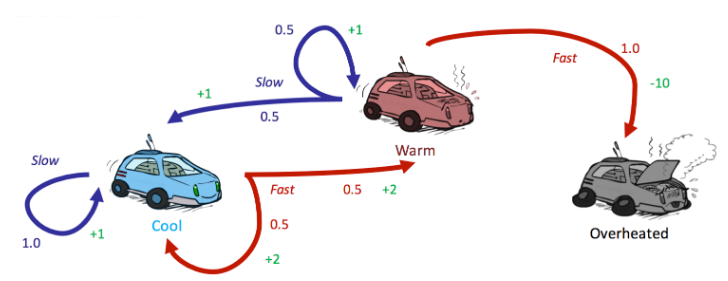
\includegraphics[width=0.65\textwidth]{../imgs/car_ex_node.png}
\end{figure}

\begin{figure}[h]
    \centering
    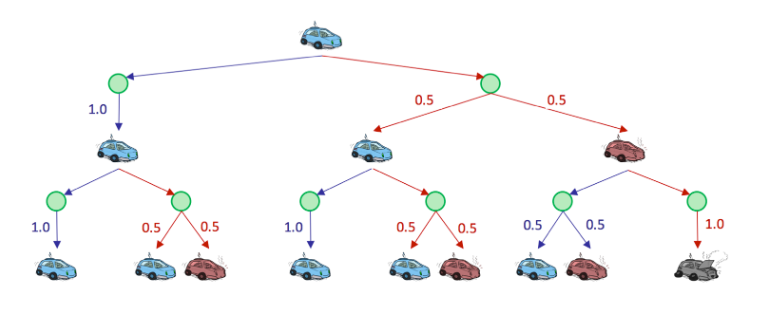
\includegraphics[width=0.7\textwidth]{../imgs/car_ex_graph.png}
\end{figure}


\subsection*{Exploitation vs. Exploration}
This is the idea of choosing between what you know and what you might learn.

\medskip

Exploration expands your knowledge; exploitation applies it. The goal is to let each one speak at the right moment.

\medskip

\textbf{Restaurant Selection}
\begin{itemize}
    \item \textbf{Exploitation:} Go to your favorite restaurant.
    \item \textbf{Exploration:} Try a new restaurant.
\end{itemize}

\textbf{Oil Drilling}
\begin{itemize}
    \item \textbf{Exploitation:} Drill at the best known location.
    \item \textbf{Exploration:} Drill at a new location.
\end{itemize}

\paragraph*{Epsilon-greedy algorithm}

The epsilon-greedy approach selects the action with the highest estimated reward most of the time
With a small probability of $\epsilon$, we choose to explore, i.e., not to exploit what we have learned so far

\begin{figure}[h]
	\centering
	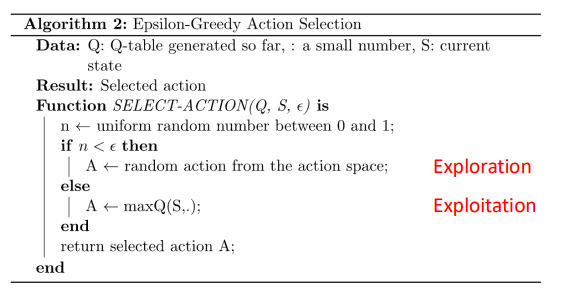
\includegraphics[width=0.5\textwidth]{../imgs/ep-greedy-algo.png} 
\end{figure}

\subsection*{Q-learning algorithm}

This algorithm converges to the optimal $Q^{*}$ under certain assumptions., The update is equivalent to gradient descent on the loss.

\begin{figure}[h]
	\centering
	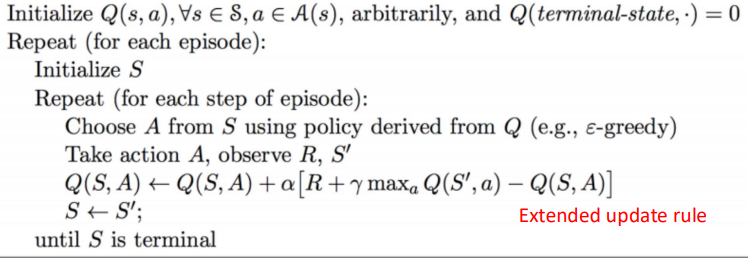
\includegraphics[width=0.5\textwidth]{../imgs/qlearn-algo.png} 
\end{figure}

Use the Bellman equation as an iterative update

\[
Q_{i+1}(s,a)
= \mathbb{E}\left[\, r + \gamma \max_{a'} Q_i(s', a') \mid s, a \,\right]
\]

\[
Q_i \;\text{will converge to}\; Q^{*} \;\text{as}\; i \to \infty
\]



\pagebreak

\subsection*{Deep Q-learning}

But traditional Q-learning has a problem, It is not scalable.

\medskip

We must compute $Q(s,a)$ for every state-action pair. If state is for example current game state pixels, this can become computationally
infeasible to compute for entire state space.

Instead we can use a function approximator to estimate Q(s,a) through a neural network!

Classical Q-learning stores values in a table, which fails for large or continuous state spaces.  
Replace the table with a parameterized function:
\[
Q(s,a;\theta) \approx Q^{*}(s,a),
\]
where $\theta$ are model parameters.  
If the function approximator is a deep neural network, the method becomes \emph{deep Q-learning}.

\medskip

\paragraph*{Target}
The Bellman target for iteration $i$:
\[
y_i = r + \gamma \max_{a'} Q(s',a';\theta_{i-1}).
\]

\paragraph*{Loss Function}

Training minimizes the squared temporal-difference error:
\[
L_i(\theta_i) = \mathbb{E}\Big[(\, y_i - Q(s,a;\theta_i) \,)^2\Big].
\]

\begin{figure}[h]
	\centering
	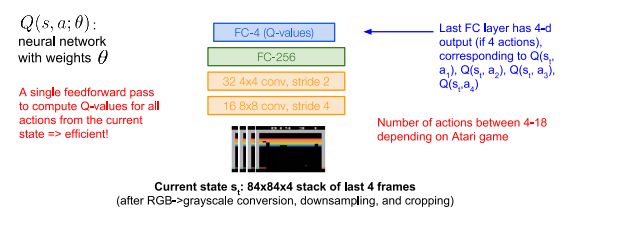
\includegraphics[width=0.85\textwidth]{../imgs/dql-arch.png} 
\end{figure}


\end{document}